\chapter{Introduction}
\label{ch:intro}

The ability to engineer and manipulate quantum states lies at the heart of modern atomic physics experiments using ultracold gases \cite{Davis1995,Anderson1995,Bradley1995,DeMarco1999,Lang2008,Ni2008}. 
Two important tools for this pursuit are Feshbach resonances \cite{Chin2010,Kohler2006} and optical lattices \cite{Bloch2008}. 
This proposal will detail our recent work building and characterizing a three-dimension optical lattice for use with ultracold and quantum degenerate gases of neutral strontium.
Furthermore, we will present the first experiment we hope to pursue with the optical lattice; the creation of Feshbach molecules using an optical Feshbach resonance. 
We will also briefly discuss other future plans such as the production of highly excited ground state Sr$_2$ dimers through adiabatic internal state transfer.

Should probably mention somewhere that this is long-range PA, in contrast to short-range stuff being explored now.

Julienne form of the corss section 6.16 in CM. Discuss how important the phase space density is, the timescale for interactions, and the complex 

\cite{Aman2018}

\section{Few-body physics}
\label{sec:few-body}

field of photoassociation in ultracold gases, wherein studies of molecular structure have revealed the most accurate descriptions of atomic interactions and have become a fundamental probe of the ultracold toolbox \cite{Jones2006}.

\section{Halo molecules}
\label{sec:halo}

Mostly studied in helium

Comes from bound state of the dirac potential. Unsure how much detail I want right here

Check out CM Juleinne pg 229. He has a ref

%% paper
Weakly bound ground-state dimers are of great interest in ultracold atomic and molecular physics. 

In the extreme case of a scattering resonance, the least-bound state represents an example of a quantum halo system \cite{jrf04} with spatial extent well into the classically forbidden region. 

Halo molecules show universality, meaning that molecular properties such as size and binding energy can be parameterized by a single quantity, the $s$-wave scattering length $a$, independent of other details of the atom-pair interaction \cite{kgj06,bha06}. 

For potentials that asymptote to a van-der-Waals form, an additional parameter, the van der Waals length $l_{\mathrm{vdW}}$, can be introduced for a more accurate description. 

Efimov trimers also exist in systems near a scattering resonance, influencing dimer and atomic scattering properties and introducing additional universal phenomena \cite{bha07,nen17}. 

Ultracold halo molecules are often associated with magnetic Feshbach resonances \cite{cgj10}, for which the scattering state and a bound molecular state can be brought near resonance by tuning a magnetic field.

This is a naturally occurring halo molecule, meaning it exists in the absence of tuning with a magnetic Feshbach resonance. 
A well-known example of a naturally occurring halo molecule is the $^4$He$_2$ dimer \cite{lmk93,sto94,kgj06}.
Moreover, the least-bound vibrational level of the ground state of $^{40}$Ca$_2$, which was recently studied using similar methods \cite{Pachomow2017a}, is similarly related to this regime.

There are important differences between halo molecules associated with magnetic Feshbach resonances and the naturally occurring halo molecule in $^{86}$Sr. 
With magnetic Feshbach resonances, the relevant scattering and bound molecular states lie on different molecular potentials, and single-photon magnetic-dipole transitions can be used to measure molecular binding energies with RF or microwave spectroscopy \cite{cgj10,cju05,thw05b}. 
Typically, this is done by first forming molecules through magneto-association and then driving bound-free or bound-bound transitions converting the halo molecule into a different state.
Other methods include spectroscopy with an oscillating magnetic field \cite{thw05b}, a modulated optically controlled Feshbach resonance \cite{chx15}, and Ramsey-type measurements of atom-molecule oscillation frequencies \cite{ckt03}. 
It is also possible to efficiently populate halo states with a magnetic-field sweep \cite{grj03} or evaporative cooling \cite{jba03} near a magnetic Feshbach resonance \cite{cgj10}. 
These are powerful techniques for manipulating quantum gases of alkali metals and other open-shell atoms, for which there are many magnetic Feshbach resonances. 
Strontium, however, due to its closed-shell electronic structure, lacks magnetic Feshbach resonances in the electronic ground state.

\section{Properties of strontium}
\label{sec:sr}

	

	\begin{figure}
		\centerline{
		\includegraphics[height=0.25\textheight]{Fig1_strontium_properties.pdf}}
		\caption{Properties of strontium. Left: Natural abundances and s-wave scattering lengths for all mixtures of Sr. Right: Simplified energy level diagram of Sr showing the relevant states used for trapping and cooling of the atomic gas}
	\end{figure} 
The experiments in this proposal will be realized using an ultracold gas of atomic strontium. Fig.\;\ref{fig:energy_level_diagram} shows all of the stable isotopes of strontium, their natural abundance, as well as their inter-particle scattering lengths. The isotopic differences in strontium have important implications for their use in certain experiments. For example, none of the bosonic isotopes of strontium ($^{88}$Sr, $^{86}$Sr, or $^{84}$Sr) display hyperfine structure since they have no nuclear spin, $\vec{I}=0$. However, the fermionic isotope $^{87}$Sr has a large nuclear spin, $\vec{I}=9/2$, which makes it an ideal candidate for exploring exotic phases of quantum magnetism \cite{Beverland2016,Cazalilla2014,Chen2015}. In the studies presented in this proposal, we are sensitive to the isotopic shifts of the bosonic photoassociation lines along the $^1S_0\!\rightarrow\!^3P_1$ transition as well as the various interspecies scattering lengths.

	\begin{figure} 
		\centerline{
		\includegraphics[height=0.4\textheight]{energy_level_diagram.png}}
		\caption{Partial energy level diagram of strontium}{Shown are the relevant transitions and decay rates utilized to perform laser cooling and spectroscopy.}
		\label{fig:energyLevels}
	\end{figure}

\begin{figure}
\label{fig:energy_level_diagram}
	\centerline{
	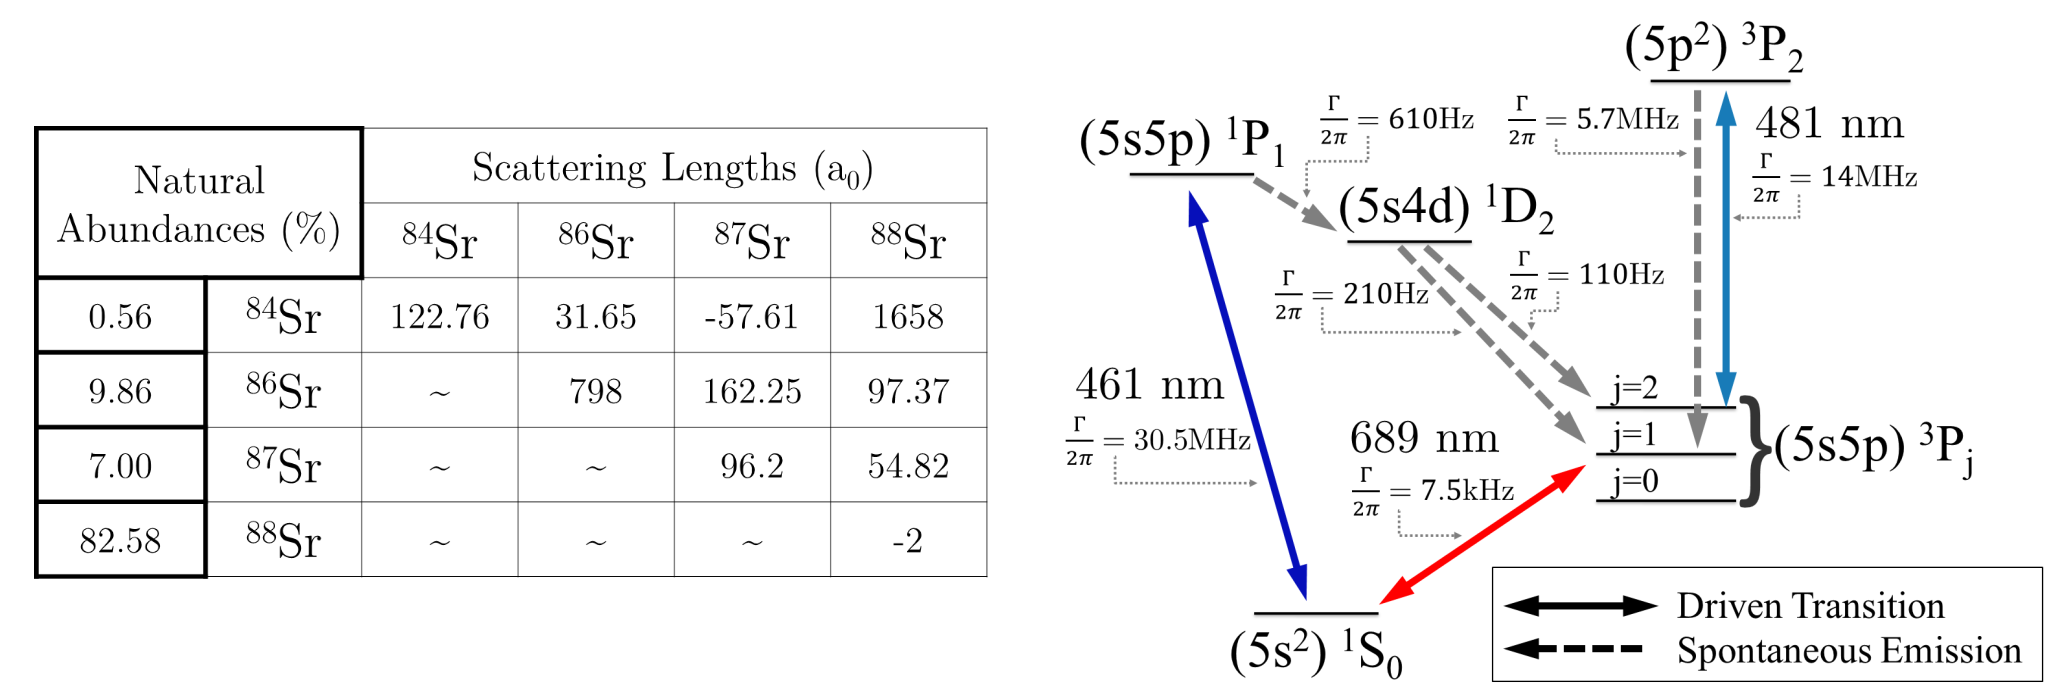
\includegraphics[height=0.25\textheight]{strontium_properties.pdf}}
	\caption{Properties of strontium}{Properties of strontium. Left: Natural abundances and s-wave scattering lengths for all mixtures of Sr. Right: Simplified energy level diagram of Sr showing the relevant states used for trapping and cooling of the atomic gas}
\end{figure} 

\section{Thesis Outline}
\label{sec:outline}

